\subsection{Muon}

Muons are distinctive signatures in final states of many physics analyses at LHC which include the Higgs analyses, SM measurements and BSM seaches and so on. 
High performance of muon reconstruction and identifications are crucial.
This section briefly describes some more details of the reconstruction, identification and isolation of muon.

\textbf{Muon reconstruction}

Muon reconstruction is firstly performed in inner detector (ID) and muon spectrometer (MS) independely as given in section~\ref{sec:track}.
The information from each individual detectors are then combined together to form the muon tracks for physics analyses.
The combined ID-MS reconstruction is developed according to several algorithm based on the information from ID, MS and calorimeters.
Four different muon types are defined\cite{Aad:2016jkr}:
\begin{itemize}
	\item \textbf{Combined (CB) muons:} a combined track is formed by using the reconstructed tracks performed independently in ID and MS with a global refit. To improve the fit quality, the hits from MS may be added to or removed from the track. The outside-in pattern recognition is utilized for the reconstruction of most muons, in which the muons are first reconstructed in MS and then extrapolated inward to match the ID track. In the meantime, the inside-out pattern is also used as a complementary method.
	\item \textbf{Segment-tagged (ST) muons:} a reconstructed track in ID is defined as muon, if it can associated with at least one track segment in MDT or CSC chambers. These ST muons are used when they can only pass across one layer of MS chambers due to their low $p_{T}$ or falling into regions with less MS acceptance.
	\item \textbf{Calorimeter-tagged (CT) muons:} a reconstructed track in ID is categorized as muon if it's matched to the energy deposit in calorimeter which is recognized with a minimum-ionizing particle. This CT muons have lowest purity amount all types of muons, but it covers the region where ATLAS muon spectrometer is only partially constructed. For the region of $|\eta| < 0.1$ and $15 GeV < p_{T} < 100 GeV$, the identification of CT muons are optimal.
	\item \textbf{Extrapolated (ME) muons:} the muon is reconstructed based only on the MS track and a loose requirement of originating from the interaction point. In general, this type of muon needs to pass at least two (three) layers of MS chambers to provide a track measurement in barrel (forward) region. ME muons are designed to extend the acceptance for muon reconstruction into the region $2.5 < |\eta| < 2.7$ where ID doesn't cover.
\end{itemize}

Before collecting those muons for physics analyses, overlap removals are performed between different muon types with the priority of CB > ST > CT, if two types of muons share the same ID track.
Besides, the overlaps with ME muons are resolved by analyzing the track hit content, and selecting the track with better fit quality and larger number of hits.

\textbf{Muon identification}

After reconstruction, the muon identification is then performed to further discriminate between signal and background, especially to suppress backgrounds from pion and kaon decays by requiring prompt muons with high efficiency and guaranteeing a robust momentum measurement.
The muon identification is defined by using the fit quality of combined track. 
The variables utilized in judgement for CB tracks include:
\begin{itemize}
	\item \textit{q/p significance}, the absolute difference between q/g (charge over momentum) of muons measured in ID and MS divided quadratic sum of their corresponding uncertainties;
	\item \textit{$\rho'$}, the absolute value of difference between the $p_{T}$ (transverse momentum) measured in ID and MS, divided by the $p_{T}$ of combined track;
	\item \textit{Nomalized $\chi^{2}$} of the combined track fit;
	\item \textit{Number of hits in ID and MS}
\end{itemize}
In addition, some new variables used for \textit{LowPt} muon working point what will be described below include\cite{Zheng:2649299}:
\begin{itemize}
	\item \textit{Momentum balance significance (MBS) } is computed as momentum difference between the ID and MS standalone measurements with respect to the uncertainty $\sigma$ on energy lost in the calorimeter system.
	\item \textit{Scattering neighbor significance (SNS)} is defined to estimated the significance of a change in trajectory along the track, expected in the presence of a hadron decaying to a muon.
	\item \textit{Scattering curvature significance (SCS)} is defined as the normalized integral of the scattering angle significances, corrected for large kinks along the trajectory.
\end{itemize}

Five selection levels are developed to satisfy the different needs for different physics goals: \textit{LowPt}, \textit{Loose}, \textit{Medium}, \textit{Tight} and \textit{HighPt}.
The \textit{Tight}, \textit{Medium}, \textit{Loose} are subsets from the tighter one to looser one.
More detailed defination of each working point is given as follow:
\begin{itemize}
	\item \textit{Loose:} this working point is designed to maximize the reconstruction efficiency while keeping good-quality of muon tracks. And they are specifically developed for reconstructing Higgs boson candidates from four-lepton final states. All four muon types are used for this selection level. The CB and ME muons passing Medium WP that will mentioned below are all included into Loose category. In addition, the CT and ST muons are restricted to $|\eta| < 0.1$ region.
In the range of $|\eta| < 2.5$, around 97.5\% Loose muons are CB muons, and about 1.5\% are CT while remaining 1\% are ST muons.
	\item \textit{Medium:} this working point is the default criteria of muon identification in ATLAS. This selection minimizes the systematic uncertainties of muon reconstruction and calibration. In this category, we only use CB and ME muons. For CB muons, at least 3 hits in at least two layers of MDT is required, except $|\eta| < 0.1$ region, in which tracks with $\geq 1$ MDT layer but $\leq 1$ MDT hole layer are allowed. For ME muons, at least 3 MDT/CSC layers is required.
Furthermore, a loose cut on the compatibility between measured momentum in ID and MS is applied to reduce the fake muons from hadrons misidentification. Besides, the q/p-significance is required to be less than 7.
	\item \textit{Tight:} this working point is used to maximize the purity of muons but with sacrifice of some selection efficiency. Only CB muons with hits in $\geq 2$ stations of MS and passing Medium caiteria are selected.
In addition, the normalized $\chi^{2}$ of combined track fit should be smaller than 8. Then, a two-dimensional cut of q/p-significance and $\rho'$ is adopted as a function of muon $p_{T}$ to ensure tighter background rejection for momentum below 20 GeV, in which the fake rate is usually higher.
	\item \textit{High-$p_{T}$:} this set of selections aims to maximize the momentum resolution for tracks with $p_{T} > 100 GeV$ region. The selection is especially optimized for searching high-mass Z' and W' resonances. CB muons satisfying Medium selection and with $\geq 3$ hits in 3 MS stations are chosen. The specific region in MS where alignment is suboptimal are removed as a precaution.
	\item \textit{Low-$p_{T}$:} this type of muon is newly designed for physics analyses with ATLAS software release version 21. It's designed to obtain a optimal muon identification with very low transverse momentum of $3 GeV < p_{T} < 5 GeV$, which is crucial for B-physics measurement in ATLAS. 
	In this muon requirement, only CB muons are used. In the range of $|\eta| < 1.3$, it requests muons hit at least one MS station; in $1.3 < |\eta| < 1.55$, a least two MS stations are required; while in region of $|\eta| > 1.55$, \textit{Medium WP} is required. In addtion, cuts are applied to suppress fakes: |MBS| < 3.0, |SNS| < 3.0 and |SCS| < 3.0.
\end{itemize}

Figure~\ref{fig:muon_id_eff} and \ref{fig:muon_id_lowpt} show the selection efficiency of different muon identification working points. For \textit{Medium}, \textit{Tight} and \textit{High-$p_{T}$:}, $Z \rightarrow \mu\mu$ events with $p_{T} > 10 GeV$ are used for measurement. 
In addition, the top plot also shows the efficiency of the \textit{Loose} selection (squares), in which the Loose and Medium selections differ significantly in region of $|\eta| < 0.1$.
For \textit{LowPt}, $J/\Psi \rightarrow \mu\mu$ events with $3 GeV < p_{T} < 10 GeV$ are used for measurement.
\begin{figure}[!htb]
  \centering
  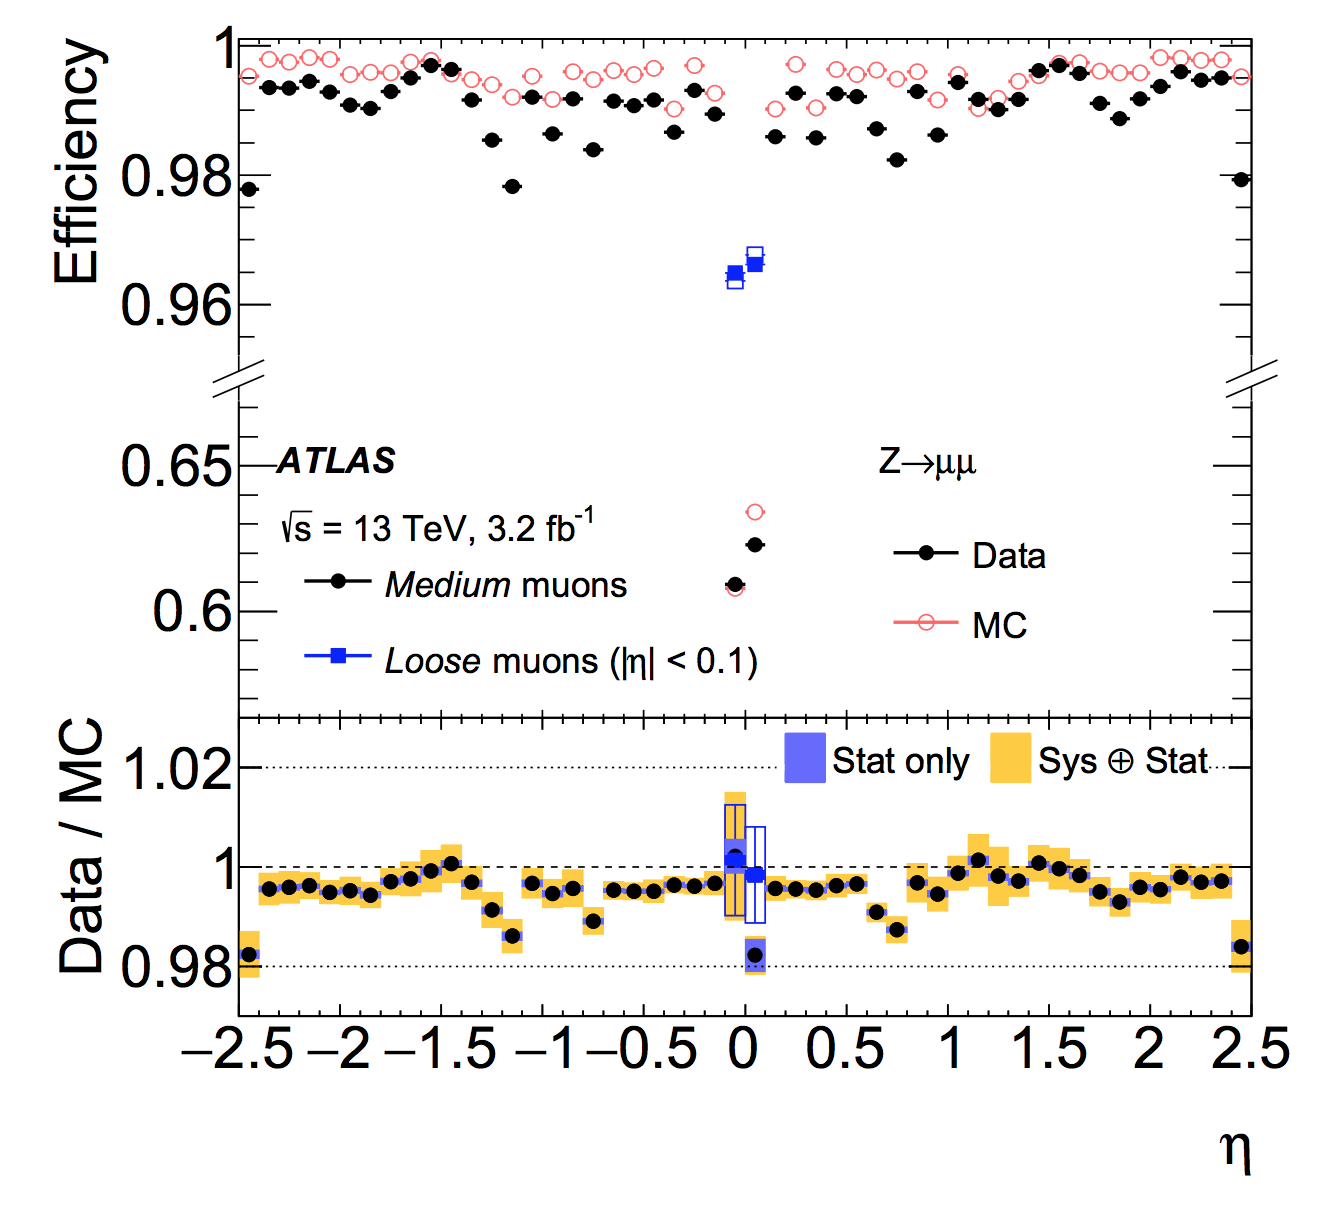
\includegraphics[width=0.42\textwidth]{figures/Simulation/muon_id_med.png} \\
  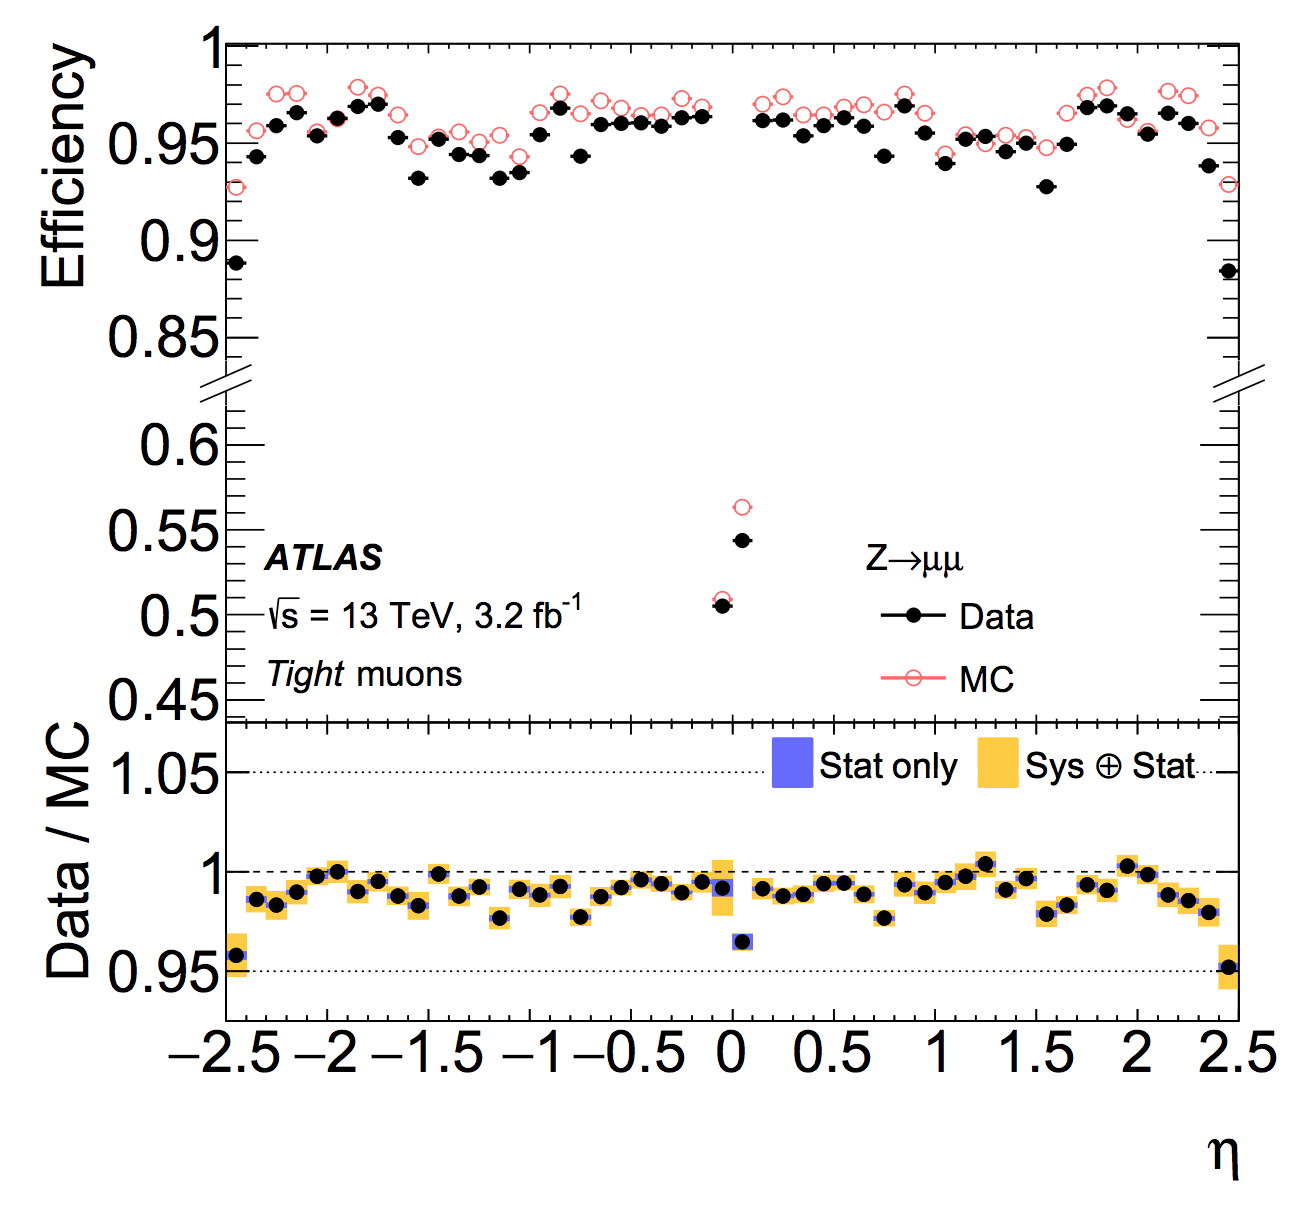
\includegraphics[width=0.42\textwidth]{figures/Simulation/muon_id_tight.png}
  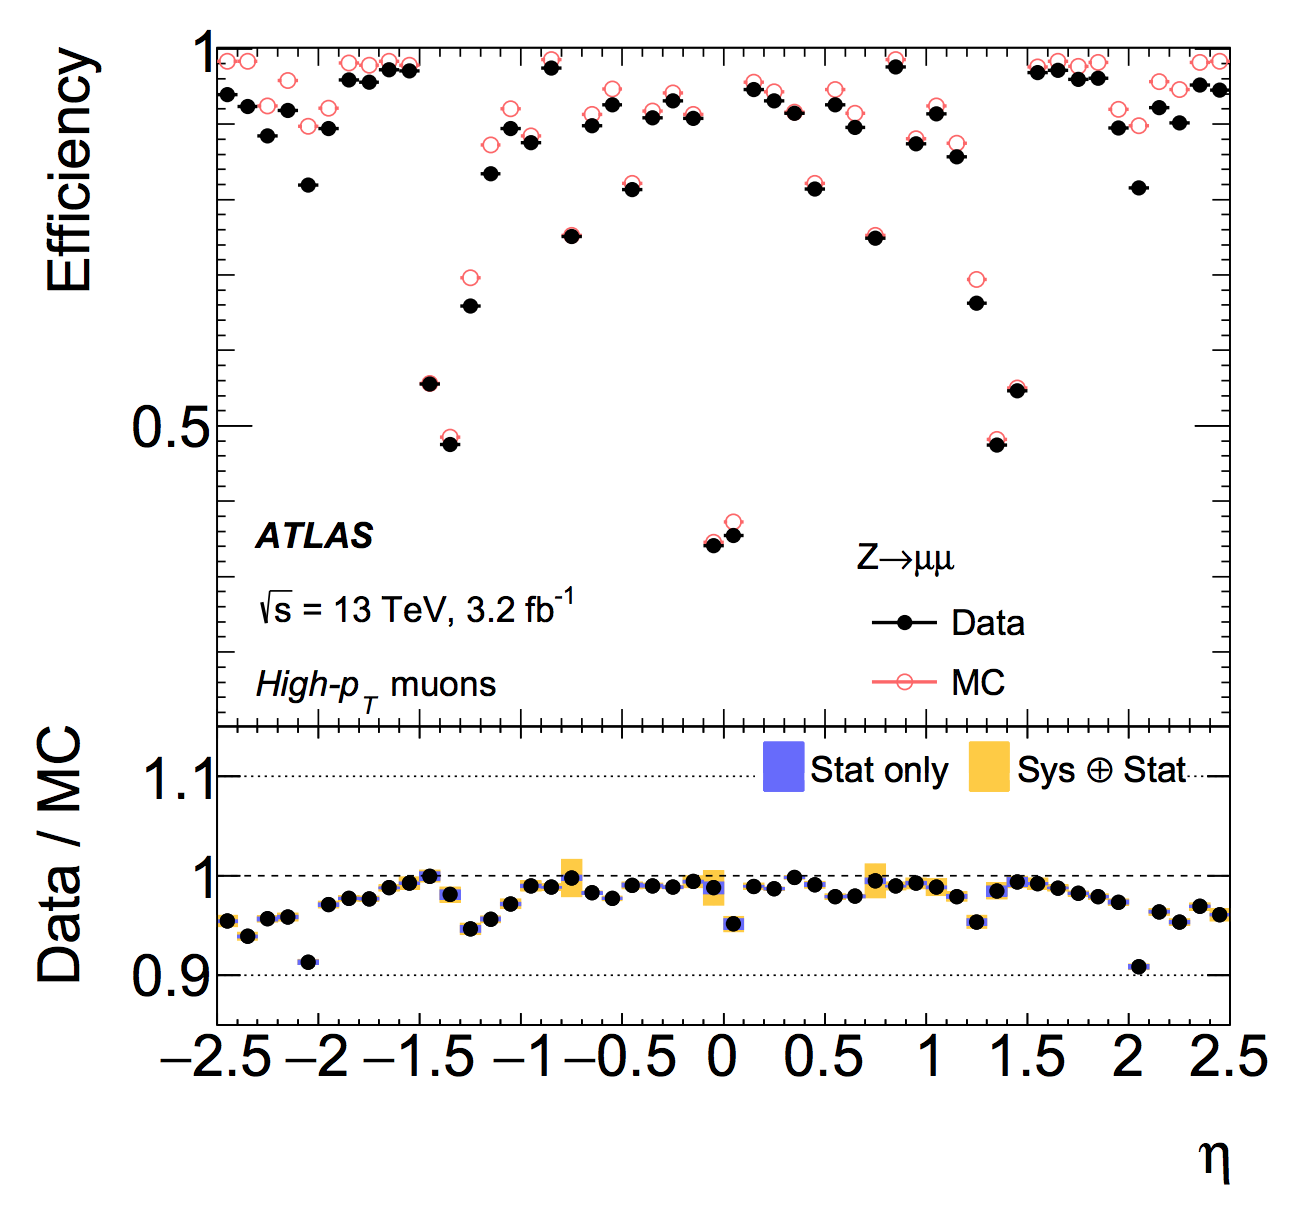
\includegraphics[width=0.42\textwidth]{figures/Simulation/muon_id_highpT.png}
  \caption{Muon reconstruction efficiency as a function of $\eta$ for: Medium (and Loose), Tight and High-$p_{T}$ working points.}
  \label{fig:muon_id_eff}
\end{figure}

\begin{figure}[!htb]
  \centering
  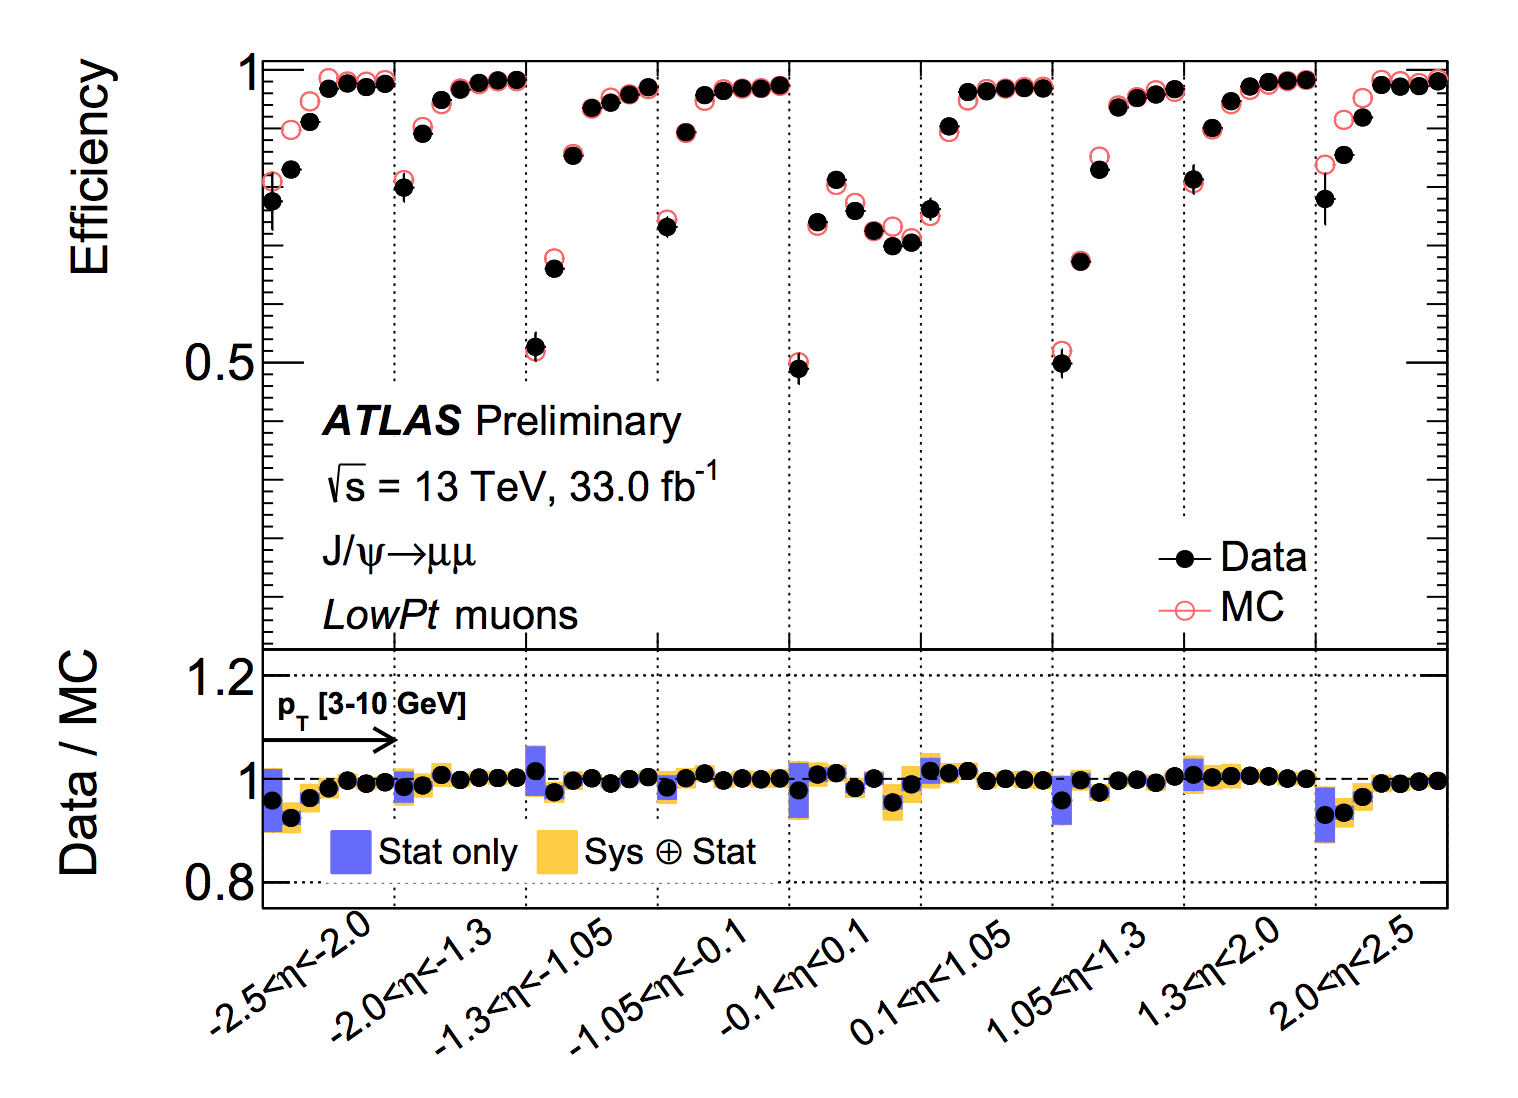
\includegraphics[width=0.5\textwidth]{figures/Simulation/muon_id_lowpT.png}
  \caption{Muon reconstruction efficiency for Low-$p_{T}$ working point as a function of $\eta$.}
  \label{fig:muon_id_lowpt}
\end{figure}

\textbf{Muon isolation}

Similar as electron, the muon isolation is used to further distinguish the prompt muon from non-prompt backgrounds.
There are also two types of isolation variables for muon:
\begin{itemize}
	\item \textbf{Calorimeter-based variable:} $E_{T}^{topocone20}$. It's defined as the sum of the transverse energy of topological clusters within a cone of size $\Delta R = 0.2$ around the candidate muon, after subtracting the contribution from the energy deposit of the muon itself and correcting for pile-up effects. The contributions from pile-up and underlying events are computed using the ambient energy-density technique\cite{CACCIARI2008119} and are corrected on an event-by-event basis.
	\item \textbf{Tracked-based variable:} $p_{T}^{varcone30}$. It's computed as the scalar sum of the transverse momenta of the tracks with $p_{T} > 1 GeV$ in a cone size of $\Delta R = min(10 GeV/p_{T}^{\mu}, 0.3)$ around the candidate muon whose transverse momenta is $p_{T}^{\mu}$ after excluding the muon track itself. This $p_{T}$-dependent cone size can help to improve the performance for muons produced in the decay of particles with a large transverse momentum.
\end{itemize}

Then the isolation selections are applied based on \textit{relative isolation variables}, 
which are computed as the ratio of the track- or calorimeter-based isolation variables to the transverse momentum of the muon.
Figure~\ref{fig:muon_iso} shows the distribution of those relative isolation variables by using $Z \rightarrow \mu\mu$ events and passing \textit{Medium} identification criteria.
\begin{figure}[!htb]
  \centering
  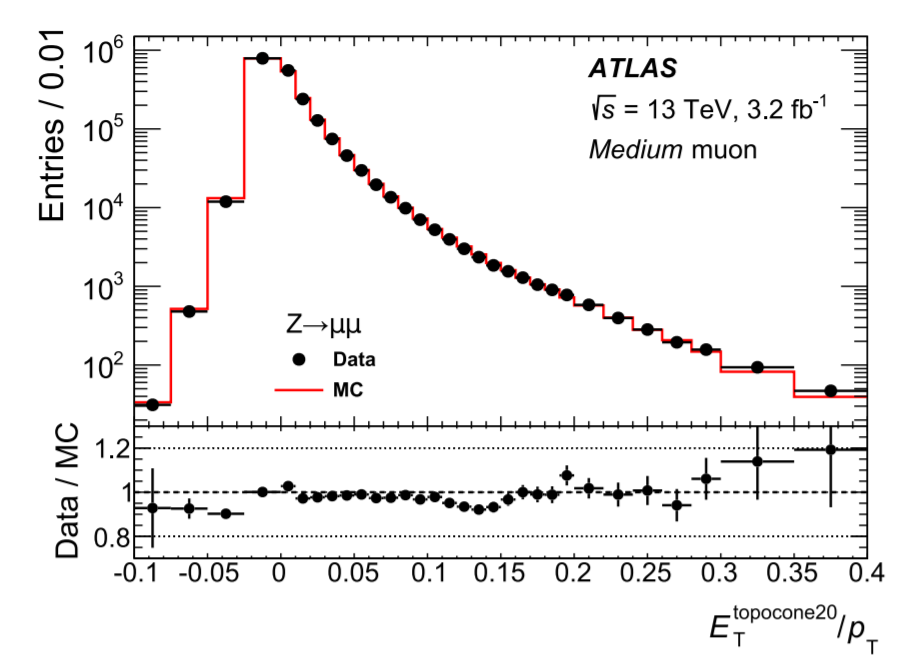
\includegraphics[width=0.42\textwidth]{figures/Simulation/muon_iso_calo.png}
  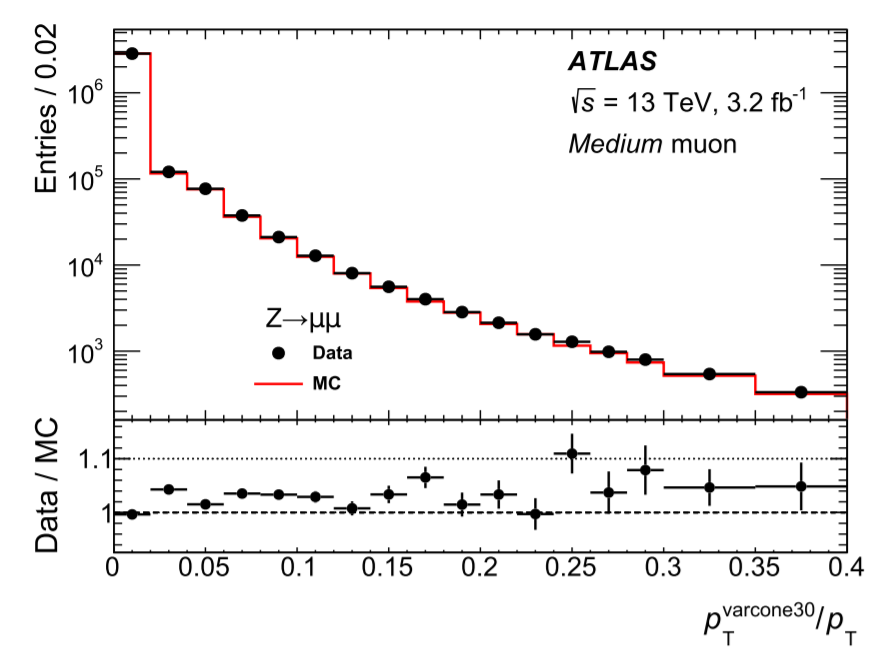
\includegraphics[width=0.42\textwidth]{figures/Simulation/muon_iso_track.png}
  \caption{Distributions of the calorimeter-based (right) and the track-based (left) relative isolation variables measured in $Z \rightarrow \mu\mu$ events. }
  \label{fig:muon_iso}
\end{figure}
